\section{Market Microstructure and Characteristics}

Market microstructure is the study of the mechanics of trading in place 
in real markets. It describes why trading occurs, the rules of trading 
and the protocols to form a trade. \citep[p. 3-4]{Has07}
Understanding market microstructure in designing an artificial market
is vital as without realistic trading settings the artifical market 
has limited practicality. In addition to microstructure, it is important
to understand the general price dynamics in order to validate representativeness
of the artifical market model. In this section, the most common 
properties of real markets and price phenomena are presented. 

% Maybe extend with behavioural aspects?

\subsection{Double Auction}
% Call-market (Itayose, Sealed-bid) vs CDA (Zaraba)

Double auction market is widely used market structure in real 
financial markets. It is a form of auction 
in which both sides of the markets, buyers and sellers, are able to 
produce quotes \citep*{Kle99}. These quotes form the order book 
which is a collection of pending bid and ask offers. A trade 
occurs between crossing and matching orders: each trade is formed between 
a bid order with a higher or equal price and an ask order with a lower 
or equal price \citep*{Ben12}. There are variations between double auction markets.
They generally differ in when the clearing process takes place 
and how the orders are matched. 
%In some implementations, such as 
%\citet*{God93}'s, a trade is formed only when a buyer and a seller 
%each agree on the exact trade price but typically the matching of crossing orders is automated.

% \subsubsection{Order Matching in Double Auction}

Main distinction between double auction market models is when
the order matching takes place. Typically, the order matching 
is continuous process occuring after the arrival of each new order but
in some markets this process takes place after a specified time interval
has passed, for example at the end of a trading day. \citep{boer05}
In auction literature, there are various terms used to describe essentially 
the same mechanics. \citet{boer05} used term 
\textit{continuous session market} for the former and \textit{call-market}
for the latter whereas \citet{ASt05} called them \textit{Itayose method}
and \textit{Zaraba method} respectively. \citet{Moc15} used term \textit{continuous 
double auction} (CDA) for the former and \textit{periodic double auction} to describe 
the same mechanics of call-markets as which they described is an extension of 
a sealed-bid auction. Sealed-bid auctions is an auction model in which the bid and ask offers
are submitted once and then the order matching is executed once. In this thesis
the terms continuous double auction and call-markets are chosen to describe
these types of markets.

In artificial market literature...
% More about Sealed-bid matching (supply-demand) and CDA matching
 
\subsection{Execution Systems}
% Quote-driven vs Order-driven
The execution systems are typically divided into two types:
quote-driven and order-driven. In quote-driven market, also known
as intermediate markets, the investors trade with prices provided 
by dealers who are part of the market organization. 
In order-driven market, also called as limit order market, 
the prices are formed according to the orders submitted by the 
investors themselves and trades are formed via automatic order matching 
or market makers. \citep{Baru17}. According to \citet{MALINOVA2013104},
the liquidity and price efficiency are generally better in order-driven 
markets. They also found out that smaller orders get better price in 
quote-driven markets due to smaller bid-ask spread 
but larger orders benefit from order-driven markets because of the lower 
execution costs. Real markets however are most often a combination
of the two \citep{boer05}.

As simulating intermediate market participants increases compexity
of the model, artificial markets with realistic quote-driven execution are rare. 
However, some artificial markets, such as \citet{SantaFe99}'s, do have some of 
the elements of quote-driven markets in a sense that the prices are driven by 
the sizes of the orders and not prices offered by the investors or traders. 
Most of the artificial markets found in the literature seem to be order-driven.


\subsection{Price Formation}
% Order book, matching and clearing
% Why we don't go deeper to quote-driven:
Price formation is direct product of the execution system in place in a market
\citep{boer05}. In order-driven markets it is direct result of the order book and
the matching algorithm in place but in quote-driven markets it
is dependent on how the intermediaries view the supply and demand of the traded
asset thus it is challenging to describe the processes from order submission
to trade formation accurately maintaining a sufficient degree of generalization.
As essentially only the order sizes are submitted to the market, the market
structure itself bears the complete responsibility to come up with prices that realistically
represent the fair price of an asset at any given time. Because of these 
factors, quote-driven was not considered for the market structure built in this
thesis and its mechanics is not discussed with more details.

% Why not the case with order-driven
On the otherhand, order-driven markets are more transparent thus there is more
to discuss about their price formation. As the limit prices are also submitted with 
the orders the supply and demand can be derived from the current state of the 
order book. Order book is a collection of bid and ask orders. There are several ways 
to match the supply and demand, or bid and ask orders, but they practically differ 
in how to distribute the surplus.

% Limit order book and terms
Limit order book is a core component in the price formation in order-driven markets.
Limit order book consists of limit orders which are simply orders that have quantity and 
a limit price stated. Limit price is the maximum price, in case of bid, or the minimum
price, in case of ask, that the order is allowed to be cleared with. In other words,
bids (asks) cannot be cleared with a price higher (lower) than the limit price stated 
in the order. There are also other types of orders, such as market and 
stop-loss orders, but these can be seen as derivatives from limit orders: 
for example, a bid (an ask) market order is essentially a limit order 
with an extremely high (low) limit price so that it does get matched 
during the clearing process regardless of the state of the order book. 
\citep{lob13}

\begin{table}
\centering
\caption{A simple representation of order book}
\label{tbl:orderbook}
\begin{tabular}{lrr}
\toprule
{} &  Bid quantities &  Ask quantities \\
price &                 &                 \\
\midrule
5.04  &               0 &             600 \\
5.03  &               0 &             500 \\
5.02  &              50 &             600 \\
5.01  &             100 &             200 \\
5.00  &             100 &             200 \\
4.99  &             250 &             150 \\
4.98  &             400 &             150 \\
4.97  &             400 &             100 \\
4.96  &             700 &               0 \\
4.95  &             500 &               0 \\
\bottomrule
\end{tabular}
\end{table}
% table.tex > \mytable

% Basics of limit order book, supply and demand etc.
A simple limit order book is presented in ~\ref{tbl:orderbook}. This table shows the
quantity of asset bidded and asked per each price level: for example, with a price of 5.00
there are 100 unit bidded and 200 unit asked. There, however, are more bids and asks that 
accept this price. Those that bid 5.01 and those that asked 4.99 would obviously also accept
this price. Therefore it is more informatic to calculate cumulative sum of bid and reverse cumulative sum of 
ask quantities and come up with total quantities of bid and ask per price level that can be matched.  
This order book with cumulative quantities is visualized in figure ~\ref{fig:lob_visual}. Cumulative bids
are renamed as demand and cumulative asks as supply as these terms are more representative in this context.
As there should not be clearable orders in continuous 
double auction's order book, except very temporarily, 
this example represents more of the order book's state in a call-market. Order book
in continuous double auction is discussed in a moment.

\begin{figure}
    \begin{center}  
        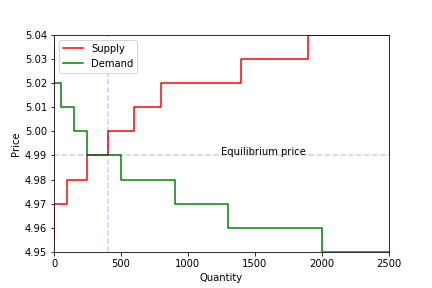
\includegraphics{plots/orderbook_visualized.png}
        \caption{Visualized order book}
        \label{fig:lob_visual}
    \end{center}
\end{figure}

% Price formation in sealed bid/call market
Call-markets typically clear at equilibrium price: at the point where
supply and demand crosses. 
To get the equlibrium price, first the maximum clearable quantity
is calculated per price level. This quantity is simply the element-wise
minimum from the supply and the demand arrays. Then the equilibrium volume
can be determined by taking the maximum from the maximum clearable quantities
per price level and equilibrium price is simply the price where the quantity
equals the equilibrium volume. A pseudocode of this algorithm is illustrated in 
algorithm ~\ref{alg:lob_equil}.

\begin{algorithm}[H]
    \SetAlgoLined
    \DontPrintSemicolon
    
    bids = sort\_ascending(bids, by price)\;
    asks = sort\_descending(asks, by price)\;
    \;
    demand = cumulative\_sum(bids, from quantity)\;
    supply = cumulative\_sum(asks, from quantity)\;
    \;
    maximum clearable per price = min\_quantity\_per\_price(demand, supply)\;
    \;
    equilibrium quantity = max(maximum clearable per price)\;
    equilibrium price = price where quantity is equilibrium quantity\;
    \KwResult{Equilibrium price and quantity}
    \caption{Pseudo algorithm for finding market equilibrium}
    \label{alg:lob_equil}
\end{algorithm}


In a continuous double auction, the matching process is slightly simpler in computation
wise as there is no need to find a common price for many orders. Only the latest arrived
order needs to be cleared, or checked for clearing, with opposing orders. Continuous
double auction does not accumulate crossing orders in similar fashion as call markets do. 
In principle, the same algorithm used in call market could be used also in continuous double auction 
but typically the surplus distribution is different. Unlike in call-markets where the surplus is often
split, in continuous double auction the surplus goes to the trader who made the latest order.
In other words, the trade prices are taken from the orders that were already in the order book.
This sort of matching could be by looping and clearing the opposing side of the order book until either
there are no more crossing orders with the newly arrived order or the new order is already cleared
completely. In case the newly arrived order is not completely cleared after depleting all the crossing
orders, it is inserted to the order book and the clearing process ends. This algorithm is illustrated in
algorithm ~\ref{alg:lob_cont}. 

\begin{algorithm}[H]
    \SetAlgoLined
    \DontPrintSemicolon
    \uIf{new order is bid}{
        asks = get\_asks(order book)\;
        price of new order = get\_price(new order)\;

        \While{(min\_price(asks) $\geq$ price of new order) \\
        \hskip\algorithmicindent\& (get\_quantity(new order) > 0)}{
            countering = filter(asks, where price $\geq$ get\_price(new order))\;
            opposite order = get\_next(countering)\;
            clear(new order, opposite order)\;
        }
    }
    \uElseIf{new order is ask}{
        bids = get\_bids(order book)\;
        price of new order = get\_price(new order)\;
        
        \While{(min\_price(bids) $\leq$ price of new order) \\ 
        \hskip\algorithmicindent \& (get\_quantity(new order) > 0)}{
            countering = filter(bids, where price $\leq$ get\_price(new order))\;
            opposite order = get\_next(countering)\;
            clear(new order, opposite order)\;
        }
    }
    \uIf{get\_quantity(new order) > 0}{
        insert\_to\_orderbook(new order)\;
    }

    \caption{Pseudo algorithm for clearing continuous double auction}
    \label{alg:lob_cont}
\end{algorithm}


% Junk?
\citet{lob13} explained thorougly the price mechanics in continuous market. I 
further generalize their explanation to include also periodical auctions.
When clearing occurs, bid orders are matched with ask orders in a way that a 
trade forms between a bid with a price p\textsubscript{b} and an ask with a price 
p\textsubscript{a} where p\textsubscript{b} $\geq$ p\textsubscript{a}. No order
should be executed with a worse price than stated in the order. However, it is likely
that not all the bids that have higher price than the lowest ask and not all the asks that
have lower price than the highest bid in the market can be matched due to the asymmetricity 
of quantity per price level. Which of these orders gets executed and what price depends on 
the details of the underlying algorithm used in the market. Before going into this with more
detail, the problem is visually described for clarification.

A simple illustration of the order book evolution is presented
in the figure ~\ref{fig:lob_evo}: the order book receives two new bids in t, bids 1 and 2.
On t + 1, clearing occurs and the bid 2 is matched with one of the equal sized best ask orders.
Bid 1 is left in the order book and becomes the best bid order. As the order prices differ
between the bid 2 and the corresponding ask, it is not entirely obvious which price to pick
for the trade: bid's price, ask's price or the average. Especially in continuous markets,
the trade price is set according to the order that was in the order book already, in this
example the ask order. % Something about supply demand price matching etc.

\begin{figure}
    \begin{center}  
        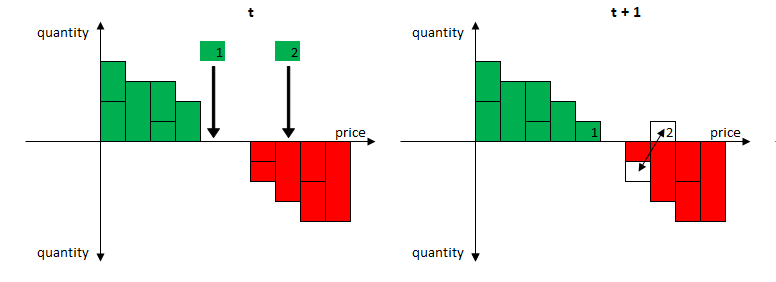
\includegraphics[width=15cm]{diagrams/lob_evolution.png}
        \caption{Evolution of a limit order book}
        \label{fig:lob_evo}
    \end{center}
\end{figure}

% Price formation in continuous settings
Price formation in continuous double auction is rather straight forward. Continuous
market do not allow clearable orders to stay in the limit order book thus the
candidates for trades can be narrowed down only to the opposing orders with better
or equal price than the newly arrived order. This is because the steps for 
clearing is conducted each time a new order arrives.





\subsection{Price Dynamics}
% Stylized facts
The price dynamics in stock markets are known to be chaotic and difficult to 
analyze. The underlying elements that play a role in the price dynamics
are constantly evolving and it still remains relatively poorly understood.
However, there are some characteristics of price behaviour that are supported
with enough empirical evidence to be considered as properties of price in
financial markets. These statistical phenomena, called stylized facts in
econometrics, have been observed in extensive amount of studies from 
different assets, markets and time periods \citep{Shakeel18}. 
% List of Stylized facts (Cont R. (2001) & Gould et al. (2013))
The price related stylized facts are according to \citet{StylizedFacts01} and \citet{lob13}:

\begin{enumerate}
    \item Fat-tailed distribution of returns: distribution of asset returns have fatter tails than normal distribution. Returns have positive excess kurtosis. 
    \par
    \begin{minipage}{\linewidth}
        \centering
        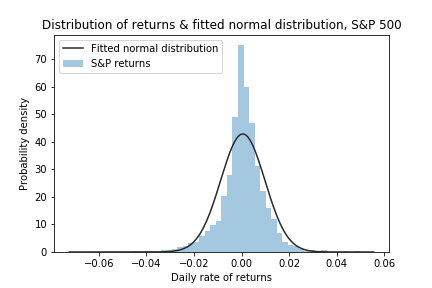
\includegraphics[width=10cm]{plots/S&P500_fat_tails.png}
        \captionof{figure}{Example of fat-tailed of returns}
    \end{minipage}

    \item Lack of autocorrelation: autocorrelation of returns in financial markets have shown to be statistically insignificant except in very short term. Previous return has no prediction power over the following. 
    \par
    \begin{minipage}{\linewidth}
        \centering
        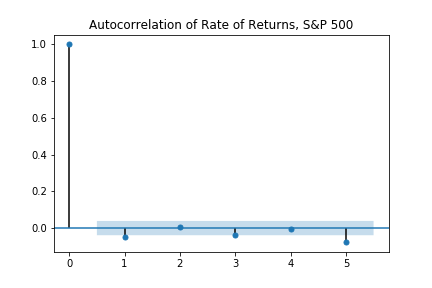
\includegraphics[width=10cm]{plots/S&P500_autocorr.png}
        \captionof{figure}{Example of absense of autocorrelation}
    \end{minipage}

    \item Volatility clusters: volatility have measured to have positive autocorrelation. Strong price movement tend to follow additional exceptional price movements forming clusters of volatility in time.
    \par
    \begin{minipage}{\linewidth}
        \centering
        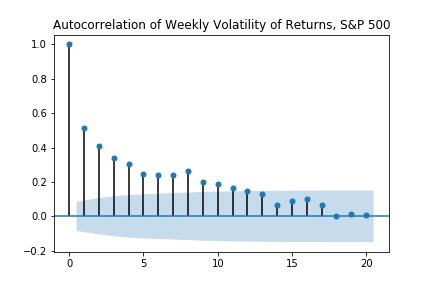
\includegraphics[width=10cm]{plots/S&P500_vola_autocorr.png}
        \captionof{figure}{Example of volatility clustering}
    \end{minipage}
\end{enumerate} 

% Something about theories of these things (explanation for the stylized facts)
% file:///D:/Opinnot/Master's%20Thesis/literature/real%20markets/price%20dynamics/TheoriesExplainingStockPriceBehavior%20(1).pdf

As has been done in the previous literature of artificial markets, the 
representativeness of the ASM built in this thesis is validated also 
using these stylized facts.